This chapter details the implementation of the automated solution proposed in Chapter \ref{chap:context}. First, an overview of the various components implemented throughout the project is given. Next, the implementation of a deep network capable of automatically extracting annual density bands present in two dimensional data is discussed. The attempts at implementing a network capable of automatically extracting the annual density bands present in three dimensions are also detailed. Then, the implementation of and reasoning behind the custom accuracy metric are discussed. Finally, the techniques used to estimate the calcification rate from the extracted boundaries are described.

\section{Overview}

A system capable of calculating of the calcification rate given only some section of density data requires the implementation of many separate subcomponents. This diagram below provides an overview of these components and outlines the order in which they were implemented and will be discussed.

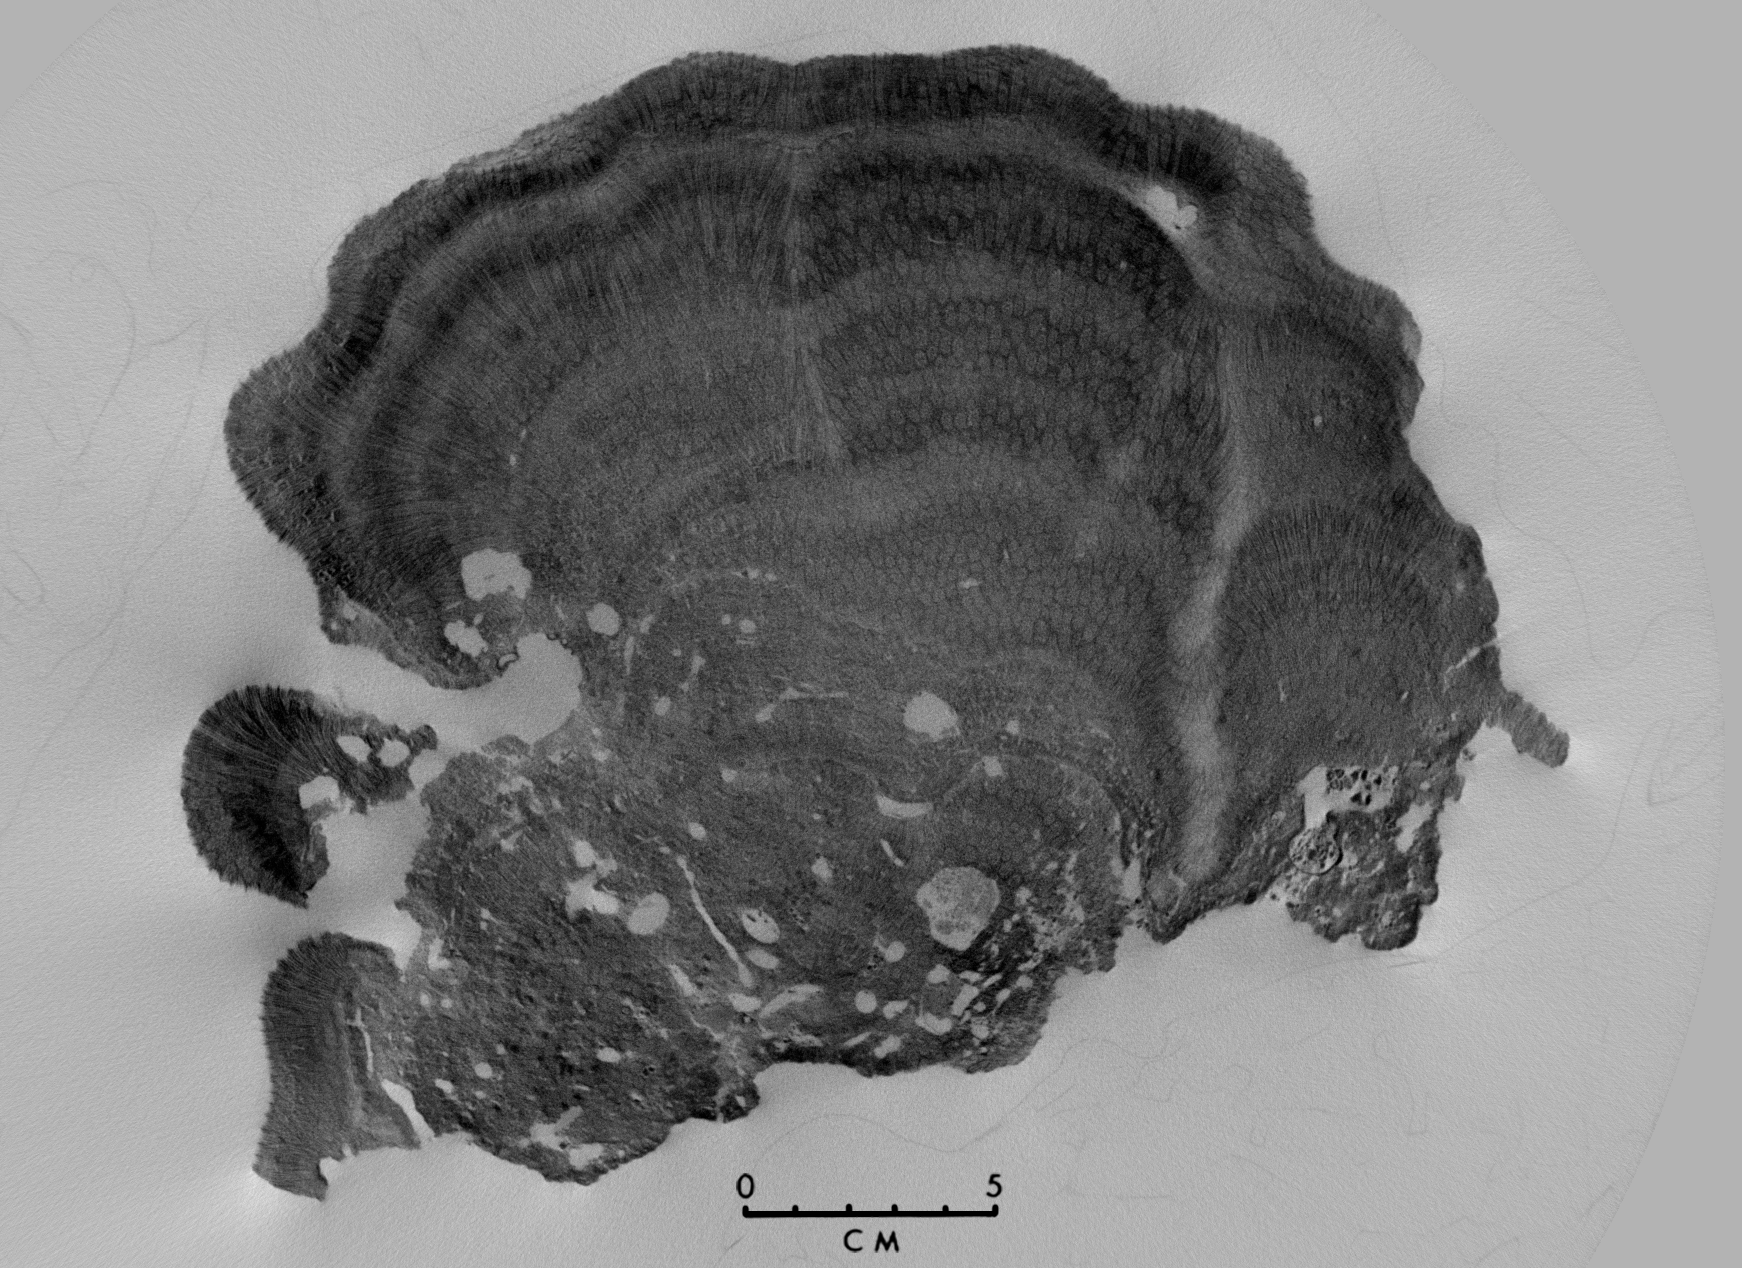
\includegraphics[width=1.02\textwidth]{images/our-coral.png}

\section{Two Dimensional Boundary Extraction}

This section outlines the steps taken to implement and train a CNN capable of extracting the annual density banding present in two dimensional data.

\subsection{Labelling the Data}

\subsection{Dataset Curation}

\subsubsection{Sliding Window}

\subsubsection{Splitting the Dataset}

\subsection{Data Augmentation}

\subsection{Architecture}

Implementation of architecture

Spatial drop out better for fully conv? \url{https://arxiv.org/pdf/1411.4280.pdf}

% From Keras docs I think
% This version performs the same function as Dropout, however it drops
% entire 2D feature maps instead of individual elements. If adjacent pixels
% within feature maps are strongly correlated (as is normally the case in
% early convolution layers) then regular dropout will not regularize the
% activations and will otherwise just result in an effective learning rate
% decrease. In this case, SpatialDropout2D will help promote independence
% between feature maps and should be used instead.

\subsection{Early Stopping and Checkpointing}

\section{Three Dimensional Boundary Extraction}

This section discusses the attempts to implement and train a CNN capable of extracting the annual density banding present in three dimensional data.

\subsection{Dataset Expansion}

\subsection{Architecture Modification}

\subsection{Data Loader Implementation}

\subsection{Three Dimensional Data Augmentation}

\section{Accuracy Metric Implementation}

\subsection{Skeletonisation}

(Show algorithm and maybe some source code?)

\subsection{The \texttt{ctypes} Module}

\section{Density Band Width Estimation}

\subsection{Point Sampling}

% {\bf A topic-specific chapter, of roughly $15$ pages} 
% \vspace{1cm} 

% \noindent
% This chapter is intended to describe what you did: the goal is to explain
% the main activity or activities, of any type, which constituted your work 
% during the project.  The content is highly topic-specific, but for many 
% projects it will make sense to split the chapter into two sections: one 
% will discuss the design of something (e.g., some hardware or software, or 
% an algorithm, or experiment), including any rationale or decisions made, 
% and the other will discuss how this design was realised via some form of 
% implementation.  

% This is, of course, far from ideal for {\em many} project topics.  Some
% situations which clearly require a different approach include:

% \begin{itemize}
% \item In a project where asymptotic analysis of some algorithm is the goal,
%       there is no real ``design and implementation'' in a traditional sense
%       even though the activity of analysis is clearly within the remit of
%       this chapter.
% \item In a project where analysis of some results is as major, or a more
%       major goal than the implementation that produced them, it might be
%       sensible to merge this chapter with the next one: the main activity 
%       is such that discussion of the results cannot be viewed separately.
% \end{itemize}

% \noindent
% Note that it is common to include evidence of ``best practice'' project 
% management (e.g., use of version control, choice of programming language 
% and so on).  Rather than simply a rote list, make sure any such content 
% is useful and/or informative in some way: for example, if there was a 
% decision to be made then explain the trade-offs and implications 
% involved.

% \section{Example Section}

% This is an example section; 
% the following content is auto-generated dummy text.
% \lipsum

% \subsection{Example Sub-section}

% \begin{figure}[t]
% \centering
% foo
% \caption{This is an example figure.}
% \label{fig}
% \end{figure}

% \begin{table}[t]
% \centering
% \begin{tabular}{|cc|c|}
% \hline
% foo      & bar      & baz      \\
% \hline
% $0     $ & $0     $ & $0     $ \\
% $1     $ & $1     $ & $1     $ \\
% $\vdots$ & $\vdots$ & $\vdots$ \\
% $9     $ & $9     $ & $9     $ \\
% \hline
% \end{tabular}
% \caption{This is an example table.}
% \label{tab}
% \end{table}

% \begin{algorithm}[t]
% \For{$i=0$ {\bf upto} $n$}{
%   $t_i \leftarrow 0$\;
% }
% \caption{This is an example algorithm.}
% \label{alg}
% \end{algorithm}

% \begin{lstlisting}[float={t},caption={This is an example listing.},label={lst},language=C]
% for( i = 0; i < n; i++ ) {
%   t[ i ] = 0;
% }
% \end{lstlisting}

% This is an example sub-section;
% the following content is auto-generated dummy text.
% Notice the examples in Figure~\ref{fig}, Table~\ref{tab}, Algorithm~\ref{alg}
% and Listing~\ref{lst}.
% \lipsum

% \subsubsection{Example Sub-sub-section}

% This is an example sub-sub-section;
% the following content is auto-generated dummy text.
% \lipsum

% \paragraph{Example paragraph.}

% This is an example paragraph; note the trailing full-stop in the title,
% which is intended to ensure it does not run into the text.
